\section{The turbine datasets and preprocessing steps }
    The data used is taken from a large Norwegian hydro electric power plant, shown in Figure \ref{fig:kvilldal} and is provided by Hymatek Controls. This plant has four identical Francis turbines, but with different maintenance history. Instead of using it as four different turbines, it is assumed that the data can be looked at as data from one turbine over a longer time period. This is of course not an ideal case, but shows one of the issues one can encounter when using data based methods. You seldom have all the data you need, and you must either add artificial data, or assume that data from other cases can be used. This is used as an assumption on how process signals from a single Francis turbine will evolve over time, as the turbine is worn down. The data collect for this project was collect during a commissioning period of the plant, meaning that it is only sampled over shorter time periods. In addition, at commissioning, a lot of tests are performed to ensure that the equipment is working as it should. One concrete example is that it can handle fast load reductions. This means that the data available most likely holds much larger variations than what would be seen for data sampled over a longer, but normal operation period.   
    
    \begin{figure}
        \centering
        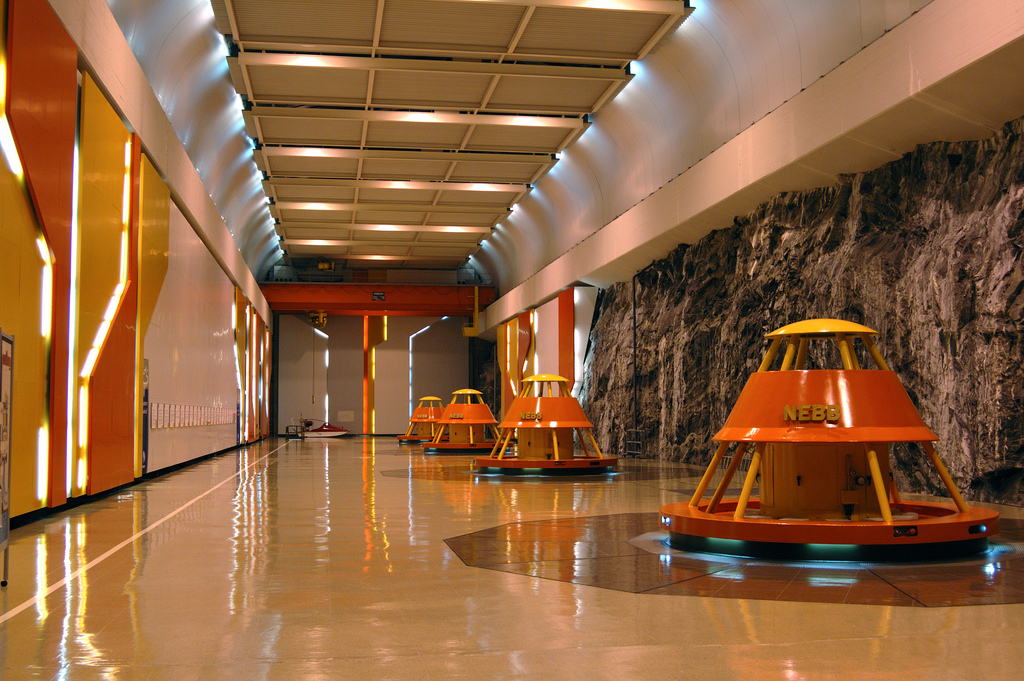
\includegraphics{figures/introduction/Kvilldal.jpg}
        \caption{Top view of the four generators at the actual plant. Courtesy of Statkraft}
        \label{fig:kvilldal}
    \end{figure}
    
    
    Table \ref{tab:variables} explains the features in the original data set.
    \begin{table}[h]
        \centering
        \begin{tabular}{|c|c|}
             \hline
             \textbf{feature} & \textbf{Interpretation}  \\ \hline
             CB pos & State of circuit breaker, open/closed  \\ \hline 
             Close & percentage(0-100\%) of closing pressure on the closing servo motor \\ \hline 
             F [Hz] & Desired output frequency in Hz \\ \hline
             F.err [Hz] & Error in output frequency in Hz \\ \hline
             Open & percentage (0-100\%) of closing pressure on the closing servo motor \\ \hline
             Sjakt & Shaft pressure (0-100\%)\\ \hline
             $Y$ [percent] & Opening of guide vanes in percent (0-100\%)\\ \hline
             $Y_{sp}$ [percent] &  Set point of opening of guide vanes in percent (0-100\%)\\ \hline
             
        \end{tabular}
        
        \caption{Table explaining the different features provided from the plant}
        \label{tab:variables}
    \end{table}
    
    
    \subsection{Original data}
        Figure \ref{fig:timeseries_A2} shows a timeseries plot  for one of the Francis generators. As can be seen the range of the Y axis is large. This is because some of the signals in the feature set have values between $0$ and $100$. This illustrates one important factor when working with data. The feature with the largest value range, will define the scale of the plot, meaning that there can be dynamics not possible to observe in this plot. This issue needs to be taken into consideration when the data is going to be used to build models. Pre-processing is a vital part of data analysis, a feature with a small range, can hold as much or more information as features with higher range. As can be seen, it is hard to interpret much from this plot. This is another very important factor to keep in mind when working with data based methods. Knowing how to make the most of the available data can make a big difference.  
        
        \begin{figure}
            \centering
            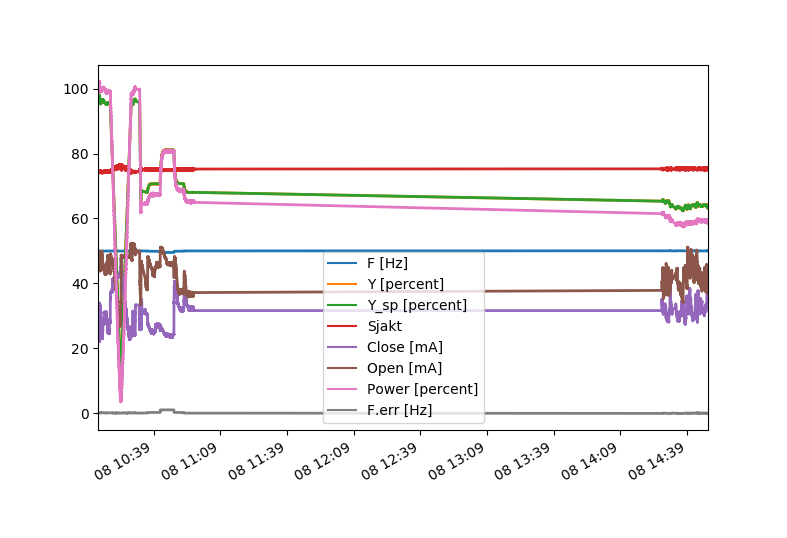
\includegraphics[width=\textwidth]{figures/data/A1_all_timeseries.png}
            \caption{Time series plot for one of the Francis turbines. Here all the original features are plotted as a function of time.}
            \label{fig:timeseries_A2}
        \end{figure}
    
    \subsection{Feature engineering}
        
        "Feature Engineering Is The Key" and "So there is ultimately no replacement for the smarts you put into feature engineering" from \cite{Domingos2012} are two very relevant quotes for this section. Good feature engineering can be the difference between success and failure when it comes to machine learning. Feeding your raw data straight into a learning algorithm is seldom the best choice. The article also discusses the difficulty with intuition in high dimensions and how generalization becomes harder as the feature set grows.     
        
        \begin{figure}
            \centering
            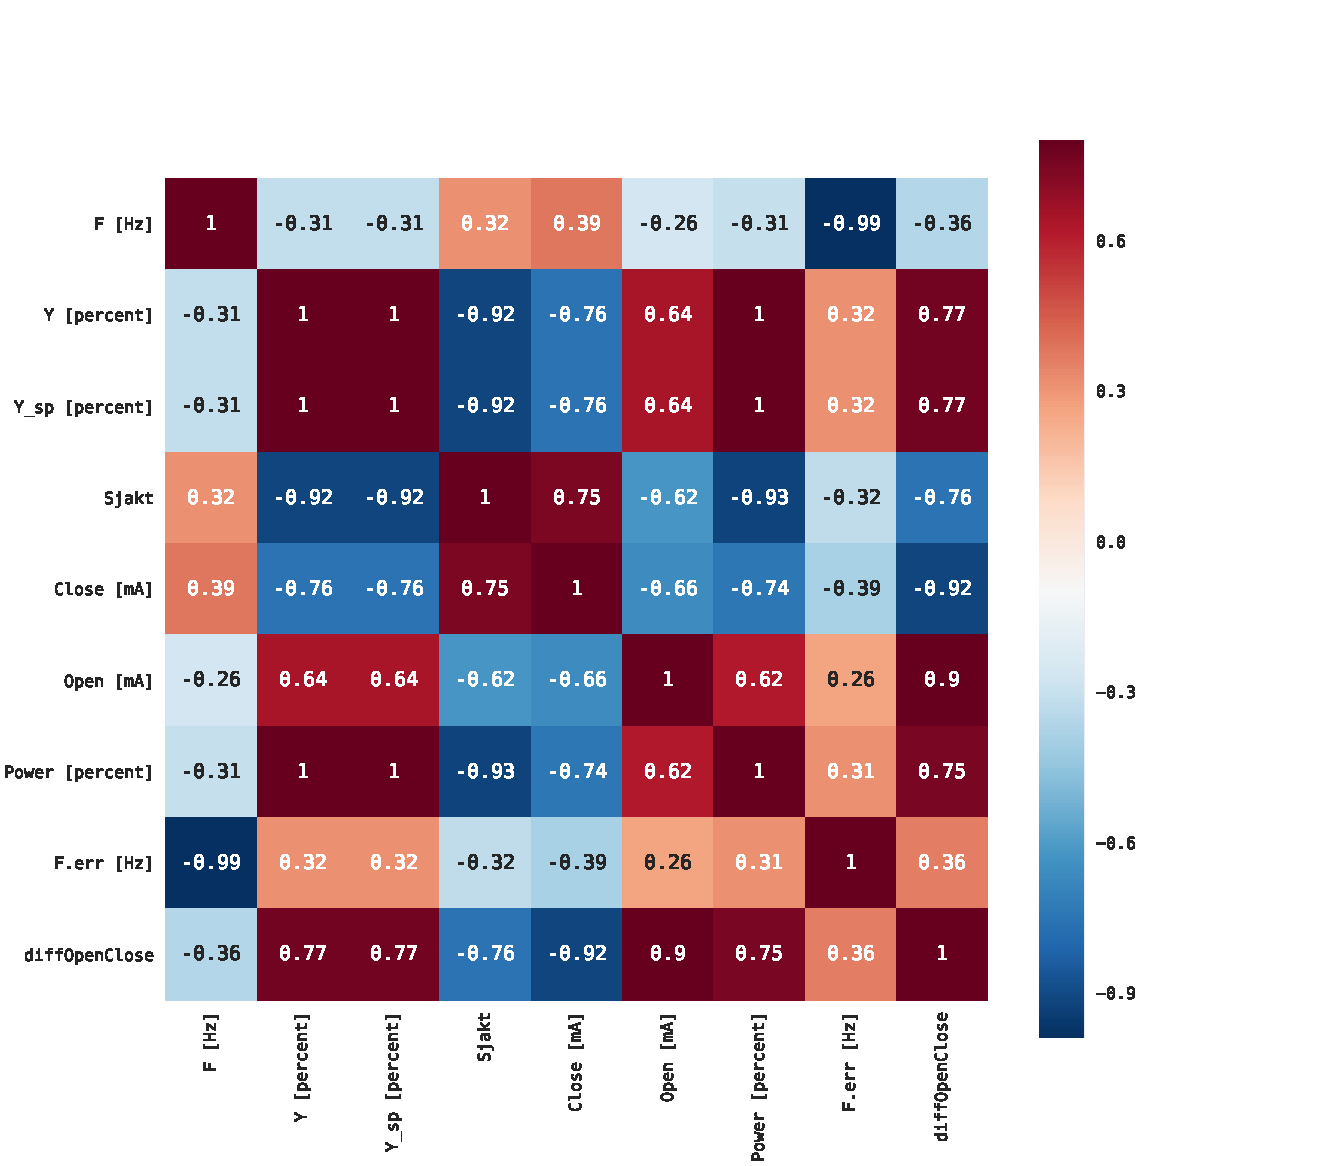
\includegraphics[width = \textwidth]{figures/data/heatmap.pdf}
            \caption{Heatmap showing the correlation between the different features in the data set.}
            \label{fig:heatmap}
        \end{figure}
    
        The heatmap in Figure \ref{fig:heatmap} shows the correlation between the different features in the data set. This is used to analyze which features that introduce new variance to the data set, and which can be explained by already existing features. The heatmap  is used to reduce the number of features that should be used in the analysis. This is known as feature extraction. The complexity of an analysis grows with the number of features, meaning that a reduced feature space, can help speed up the modeling. In the figure, where each column meets each row, a square is formed. The color and value of that square explains how the two features are correlated. A red color with a number close to one indicates that the two features are positive correlated. A dark blue color with a value close to minus one indicates negative correlation. Whine and close to zero indicate no correlation.  
        
        As mentioned in the introduction, the goal is to classify the condition of the guide vanes. \textbf{This is found as function of the differential pressure of the open and closing servos}. Hence $Y$, open and close should be the most interesting features in this data set. As can be seen, $Y$ and $Y_{sp}$ are strongly correlated. This is as expected, since the control system is constantly working to keep $Y$ as close to $Y_{sp}$ as possible. Hence, dropping one of these features in the further analysis will not reduce the amount of information found in the data set. A new feature is added, the difference between $open$ and $close$. This is done to see if the two features can be reduced to one. As can be seen in the column for the new feature $diffOpenClose$ in the heat map, it is strongly correlated with open, and strongly negatively correlated with closing. It is therefore chosen as a substitute for the two original features. The two frequency features are observed to have small correlations with both opening and the new $diffOpenClose$ feature. They are however left out of the feature set. The frequency of the power generated by the turbine is controlled by a set point, and hence it makes sense that it holds little information about the degradation of the guide vanes inside the turbine. $Sjakt$ is the last feature to analyze. As can be seen in the figure, it is negatively correlated with both $Y$ and $diffOpenClose$. It might hold some interesting information for the analysis, but the benefit of keeping the feature space in two dimensions, is weighted higher, and hence it is also left out. From now on the data set is only containing $Y$ and $diffOpenClose$ as features.    
        
    \subsection{Splitting the data}
        As mentioned in the introduction, the state of the guide vanes is by the current approach estimated by analyzing a servo indication of the turbine. Therefore the servo indication is separated from the rest of the commissioning data. This enables analysis on the pure servo indication. The two different datasets will be referenced as \textbf{commissioning} and \textbf{servo indication} from now on. This also introduce the possibility to compare if it is possible to extract the servo indication information from a commissioning or not. Figure \ref{fig:start_up_4} shows the commissioning data for the four different data sets. The $Y$ axis named delta force, is the diffOpenClose feature added to the data set. As can be seen, A3 is the set with lowest differential and A4 is the one with the highest. Figure \ref{fig:start_up_1}, shows the four different data sets plotted against each other. One clear issue is that the A1 set does not span as far as the three others. This is again an example of issues when working with real data. Sometimes one does not have available what one should have. From Figure \ref{fig:start_up_4} and \ref{fig:start_up_1} one can clearly now see the influence of feature engineering compared to Figure \ref{fig:timeseries_A2}. Figure \ref{fig:servo_indication_all} shows the data from the servo indications for the four different turbines. Here one can more easily interpret the four sets in one plot, so a plot for each one individually is left out. One important thing to notice is that the servo indications holds only the information one actually want when estimating the state of the guide vanes, there are only samples that lay on the boundary. Compared to the commissioning sets seen in Figure \ref{fig:start_up_4} where there are a lot of samples located inside the boundary. 
        
        \begin{figure}[h]
            \centering
            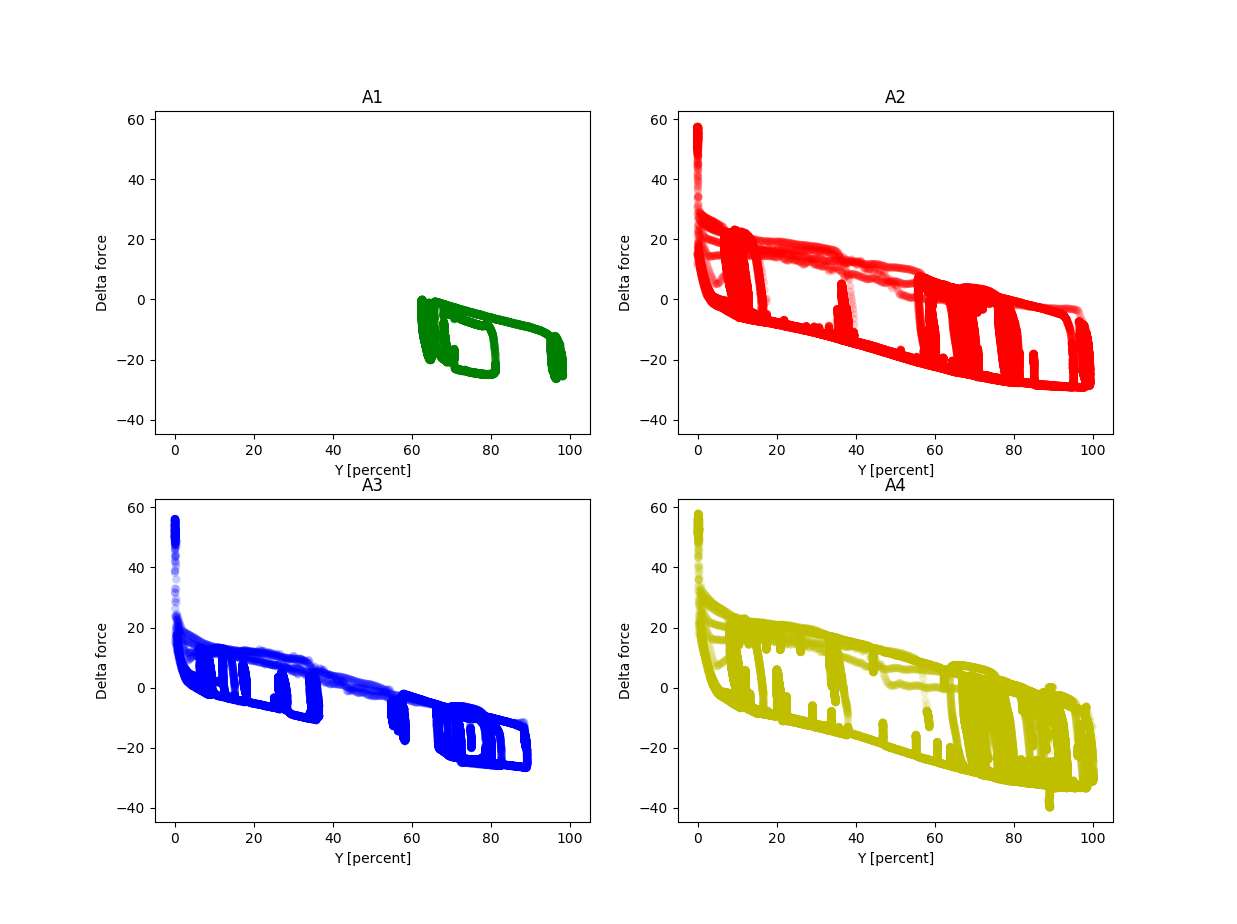
\includegraphics[width = \textwidth]{figures/data/start_up_all.png}
            \caption{Commissioning data for the four turbines. High non linearity can be observed in the left part of the subplots for A2-A4. Also notice that the test data for A1 is very reduced compared to the others. The numerical values of the delta force axis does not correspond to any SI units, it just serves as a factor that can be used to separate the different sets}
            \label{fig:start_up_4}
        \end{figure}
        
        \begin{figure}[h]
            \centering
            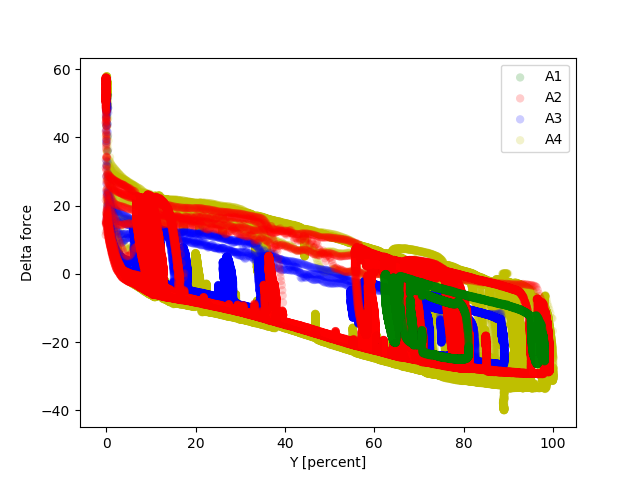
\includegraphics[width = 0.6\textwidth]{figures/data/start_up_all_one_plot.png}
            \caption{The four test sets plotted in the same window. Due to the large amount of samples, and the overlapping samples some of the turbine samples are hidden. It is however possible to verify that A4 is the set with highest delta force, and A3 ist the one with lowest.}
            \label{fig:start_up_1}
        \end{figure}
    
        \begin{figure}[h]
            \centering
            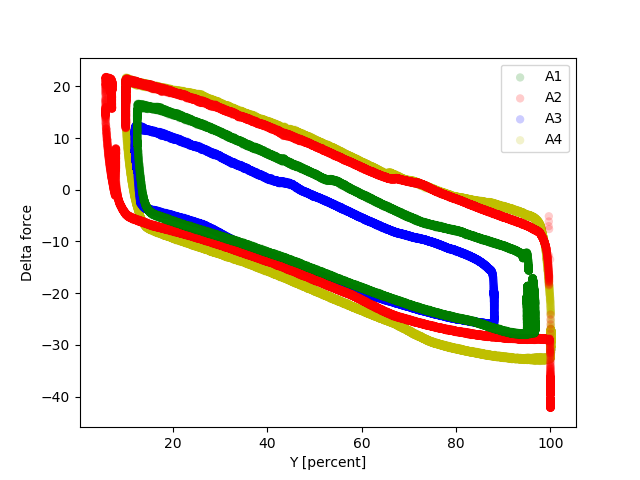
\includegraphics[width = 0.6\textwidth]{figures/data/servo_indication_all_one_plot.png}
            \caption{The four servo indications plotted in the same window. The pure servo indication does not contain any samples inside the boundary area, making the scale of the different turbine data sets easier to interpret. A3-A1-A2-A4 from good to poor.}
            \label{fig:servo_indication_all}
        \end{figure}
        
        
    \subsection{Preprocessing}
        Once the feature space is reduced and the data sets are split, the next step is to preprocess the data, making sure that it is suitable for a learning algorithm. The data for the $4$ different cases comes in several .csv files, sampled during commissioning. I want to thank my supervisor Anders from Hymatek for providing a Python API that reads the files from .csv into python. Figure \ref{fig:start_up_4} shows as mentioned in its caption high nonlinearity in the left part of the plot. This makes the boundary more complex, and it holds little information about the guide vanes. Therefore the samples that lay in this space are removed from the dataset.    
        
        
        \subsubsection{Downsampling}
            The sample rate for the data is 50 Hz, meaning that every $20$ms a new sample is taken. Even for a shorter time period, this yields an enormous amount of samples. Figure \ref{fig:downsample} shows Kde plots for the original and down sampled data set for turbine A4. Kde or kernel density estimation is a way to estimate the probability density function of variable or feature. The Kde for both features are shown above and to the right of the plots. The red color around the samples indicates where the highest density of samples are. This means the plots clearly show where most of the data is located. 
            
            The left figure shows the plot for the commissioning dataset for turbine $4$. The original commissioning set has a sample size of $133700$ samples. The right plot has the sample rate reduced to $1$s, reducing the sample set size to $10756$. Note that there are some holes in the sampling, meaning that there are seconds which not have 50 samples. This is the reason for the unbalance between the number of samples in the original vs the down sampled dataset. As can be seen in Figure \ref{fig:downsample} the shape of the  correlation curves are very similar for both plots. One can also verify that the contours of the original set is still a part of the down sampled plot. This means that even if the amount of data is reduced, it still includes the same shape and density as the original data. Therefor the reduced data sets are the ones used for the analysis. The corresponding plots for the three remaining data sets are found in \textbf{appendix A}. The p value in the upper right corners, indicates the probability of an uncorrelated dataset producing a dataset that has a pearsonr correlation as high or higher as the set. The pearsonr measures the pearsonr correlation, which is a a measure of the linear correlation between the two features    
        
            \begin{figure}[h]
                \begin{minipage}[b]{0.5\linewidth}
                    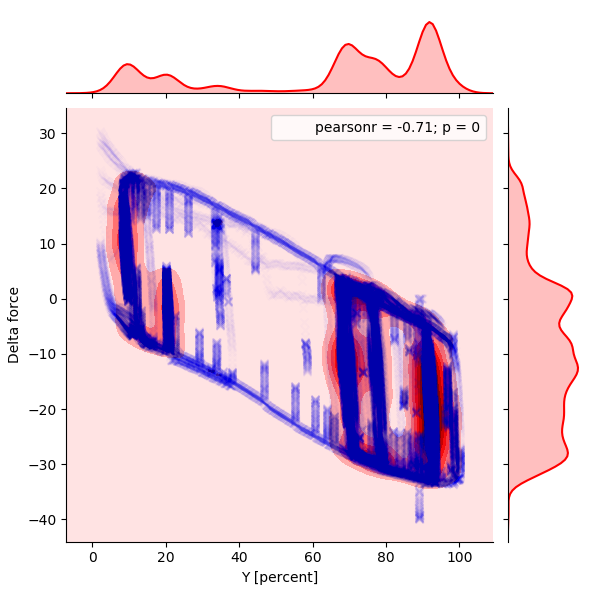
\includegraphics[width=1\linewidth]{figures/data/kdePlot_noServo_A4.png} 
                \end{minipage}
                  \hfill
                  \begin{minipage}[b]{0.5\linewidth}
                    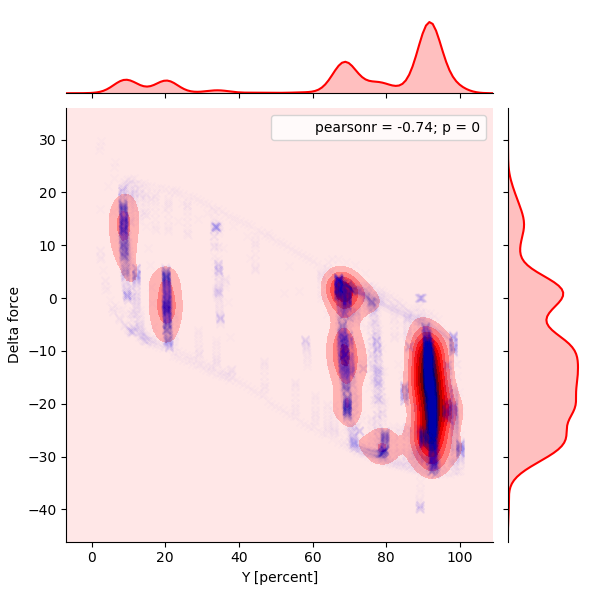
\includegraphics[width=1\linewidth]{figures/data/kdePlot_reduced_noServo_A4.png} 
                \end{minipage} 
                \caption{Kde plots for original commissioning data, and down sampled commissioning data for turbine $4$.}
                \label{fig:downsample}
            \end{figure}
        
            For the servo indication sets, the Kde plot for A4 is seen in Figure \ref{fig:kde_servo}. As can be seen here the data is uniformly distributed around the boundary. The size of the servo indication sets are also much smaller (around $30000$ samples) than the test sets, and they are therefore kept without re-sampling. The plots for the three remaining turbines can be found in \textbf{appendix A}.  
            
            \begin{figure}[h]
                \begin{minipage}[b]{0.5\linewidth}
                    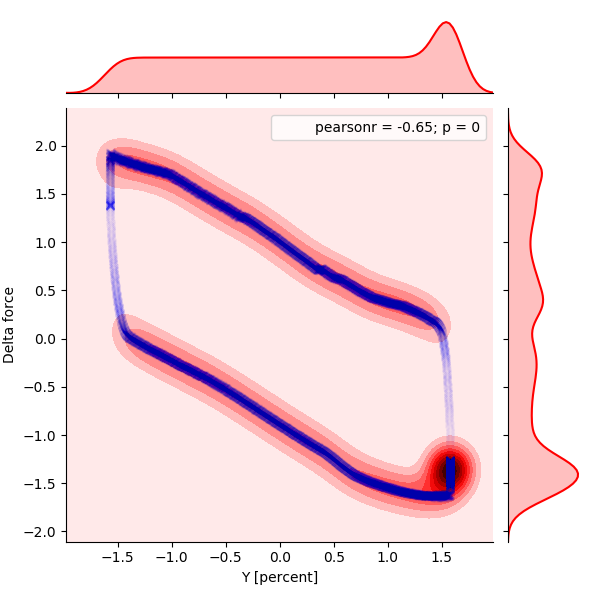
\includegraphics[width=1\linewidth]{figures/data/kdePlot_servoindication_A4.png} 
                \end{minipage}
                  \hfill
                  \begin{minipage}[b]{0.5\linewidth}
                    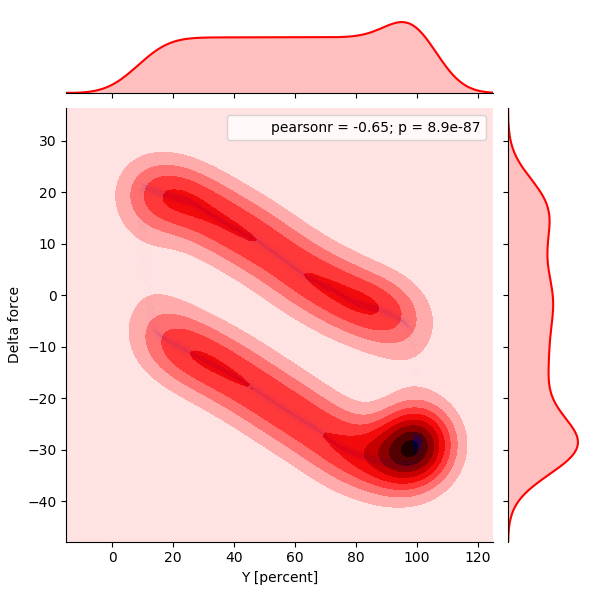
\includegraphics[width=1\linewidth]{figures/data/kdePlot_reduced_Servo_A4.png} 
                \end{minipage} 
                \caption{Kde plots for original servo indication data, and down sampled servo indication data for turbine $4$.}
                \label{fig:kde_servo}
            \end{figure}

        \subsubsection{Scaling}
            The final step of the preprocessing is to scale the each feature. First all samples are mean centered, and they are then scaled to unit variance. The result is shown in Figure \ref{fig:start_up_reduced_4}. Notice that the range of the $X$ and $Y$ axis are now approximately the same. The non linearity seen in Figure \ref{fig:start_up_4} is also removed. The data is now ready for analysis.     
            
            
        
            \begin{figure}[h]
                \centering
                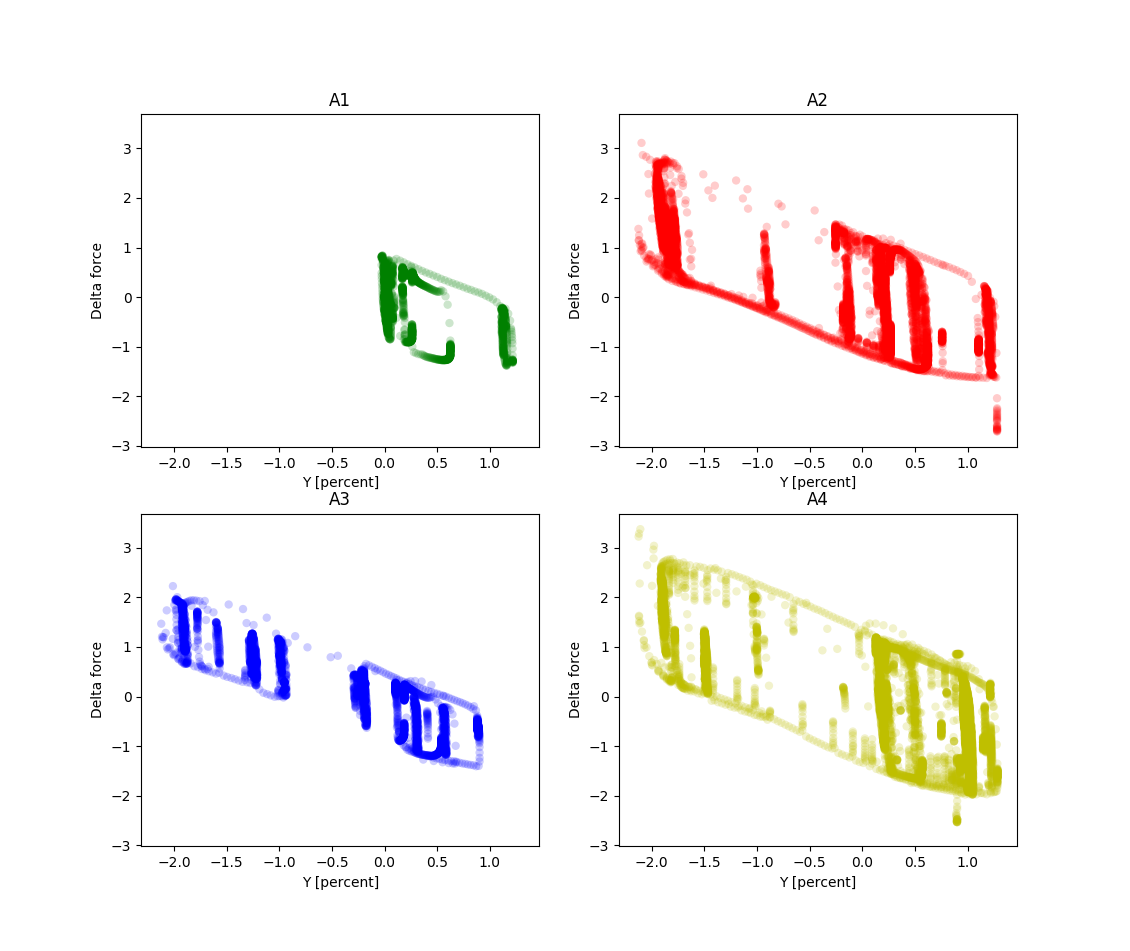
\includegraphics[width = \textwidth]{figures/data/start_up_reduced_4.png}
                \caption{The reduced commissioning data set, here each sample is given an alpha = 0.2, this means that the intensity of the color is high where several samples overlap}
                \label{fig:start_up_reduced_4}
            \end{figure}